% 绕轴旋转矩阵
% 线性代数|矩阵|矢量|数乘|内积|叉乘|空间旋转矩阵|绕轴旋转矩阵|匀速圆周运动|线速度

\pentry{空间旋转矩阵\upref{Rot3D},圆周运动的速度\upref{CMVD}}

直角坐标系中,某点 $\bvec r=(x,y,z)\Tr$ 以单位矢量 $\uvec A=(A_x, A_y, A_z)\Tr$ 为轴按右手定则%未完成 链接
转动 $\theta$ 角的得到的点 $\bvec r'=(x',y',z')\Tr$ 可用矩阵乘法计算
\begin{equation}
\bvec r' = \mat R_\theta \bvec r
\end{equation}
其中 $\mat R_\theta$ 为\bb{绕轴旋转矩阵}
\begin{equation}
\mat R_\theta =
\begin{pmatrix}
a A_x^2 + c & a A_x A_y - s A_z & a A_x A_z + s A_y\\
a A_y A_x + s A_z & a A_y^2 + c & a A_y A_z - s A_x\\
a A_z A_x - s A_y & a A_z A_y + s A_x & a A_z^2 + c
\end{pmatrix}\end{equation}
其中
\begin{equation}
c = \cos\theta \qquad s = \sin\theta \qquad a = 1 - \cos\theta
\end{equation}
事实上, 数学上更规范的做法是用四元数\upref{QuatN}表示该矩阵.

\subsection{推导}
推导的思路是用 $\uvec A$ , $\bvec r$ 和 $\theta $ 三个已知量经过数乘,内积\upref{Dot}和叉乘\upref{Cross}三种运算,表示出旋转后的矢量 $\bvec r'$,再拆成三个分量,即可得到线性变换,进而写出矩阵. 注意该思路与推导平面旋转矩阵\upref{Rot2D} 的思路不一样.
\begin{figure}[ht]
\centering
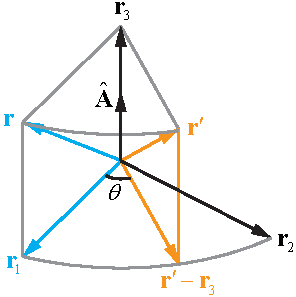
\includegraphics[width=5.5cm]{./figures/RotA1.pdf}
\caption{绕轴旋转矩阵的推导}
\end{figure} 

如图, $\bvec r$ 绕单位矢量 $\uvec A$ 旋转后得到 $\bvec r'$.  $\bvec r$ 在 $\uvec A$ 方向的分量为   
\begin{equation}\label{RotA_eq4}
\bvec r_3 = (\uvec A \vdot \bvec r)\uvec A
\end{equation}
在与 $\uvec A$ 垂直方向的分量为
\begin{equation}\label{RotA_eq5}
\bvec r_1 = \bvec r - \bvec r_3
\end{equation}
为了构成一组正交基底,令
\begin{equation}\label{RotA_eq6}
\bvec r_2 = \uvec A \cross \bvec r_1
\end{equation}
则 $\bvec r_2$ 相当于 $\bvec r_1$ 绕 $\uvec A$ 旋转 90°. 现在有了正交的 $\bvec r_1$ , $\bvec r_2$  就可以表示出 $\bvec r_1$ 绕 $\uvec A$ 旋转 $\theta$ 角后的结果
\begin{equation}
\bvec r' - \bvec r_3 = \bvec r_1\cos \theta  + \bvec r_2\sin \theta
\end{equation}
即
\begin{equation}\label{RotA_eq8}
\bvec r' = \bvec r_1\cos \theta  + \bvec r_2\sin \theta  + \bvec r_3
\end{equation} 
将\autoref{RotA_eq4} \autoref{RotA_eq5} \autoref{RotA_eq6} 代入\autoref{RotA_eq8}, 即可求出 $\bvec r'$ 关于 $\uvec A$ , $\bvec r$ 和 $\theta $ 的矢量表达式. 把结果写成分量的形式,化简可得到 $x',y',z'$ 关于 $x,y,z$ 的线性变换与系数矩阵\upref{Mat}.

\subsection{由旋转矩阵推导出匀速圆周运动的线速度} 

我们可以用旋转矩阵得到 $\bvec v = \bvec \omega  \cross \bvec r$ (\autoref{CMVD_eq5}\upref{CMVD}), 这也验证了旋转矩阵的正确性.

在无穷小的时间 $t$ 内,点 $P$ 绕轴转过 $\theta $ 角,则 $\theta  = \omega t \to 0$, 此时有 $\sin\theta  \to \theta $ 和 $\cos\theta  \to 1$. 旋转矩阵变为
\begin{equation}
\mat R_\theta =
\begin{pmatrix}
1 & -A_z\theta & A_y \theta\\
A_z \theta & 1 & -A_x \theta\\
-A_y \theta & A_x \theta &1
\end{pmatrix}
\end{equation}
下面 $\mat R_\theta$ 乘以某点的列矢量,得到变换后的坐标,再减掉变换前的坐标,得位移矢量 $\bvec s$
\begin{equation}\ali{
\bvec s &= \bvec v t\\
&= \pmat{1 & -A_z\theta & A_y\theta\\A_z\theta & 1 & -A_x\theta\\-A_y\theta & A_x\theta & 1} \pmat{x\\y\\z}
-\pmat{1&&\\&1&\\&&1} \pmat{x\\y\\z}\\
&= \theta \pmat{0 & -A_z & A_y\\A_z & 0 & -A_x\\-A_y & A_x & 0}\pmat{x\\y\\z}\\
&= \theta\uvec A\cross\bvec r
= \qty(\bvec \omega t) \cross \bvec r
}\end{equation} 
两边除以 $t$,得 $\bvec v = \bvec \omega  \cross \bvec r$. 
